\documentclass[12pt]{article}
 
\usepackage[margin=.75in]{geometry} 
\usepackage{amsmath,amsthm,amssymb}
\usepackage{fancyhdr}
\usepackage{color}
\usepackage{tikz,graphicx}
	\usetikzlibrary{arrows,plotmarks,shapes}
	



\newenvironment{problem}[2][Problem]{\begin{trivlist}
\item[\hskip \labelsep {\bfseries #1}\hskip \labelsep {\bfseries #2.}]}{\end{trivlist}}


%%%%%%Header/Footer%%%%%%%

\pagestyle{fancy}

\lhead{\LARGE \textbf{Probability Activity}}
\chead{} 
\rhead{\thepage}

\lfoot{} 
\cfoot{} 
\rfoot{}
\renewcommand{\headrulewidth}{0.4pt} 
\renewcommand{\footrulewidth}{0pt}

%%%%%%%%%%%%%%%%%%%


\begin{document}
\noindent
Consider the following spinner for this activity.

\begin{center}
\begin{tikzpicture}[scale=5]
\draw(0,0) circle (1.414cm);	
\draw (-1.41,0) -- (1.41,0);
\draw (0,1.41) -- (0, -1.41);
\end{tikzpicture}
\end{center}

\vspace{-15.80cm}

\begin{center}
\begin{tikzpicture}[rotate=45, scale=5]
\draw(0,0) circle (1.414cm);	
\draw (-1.41,0) -- (1.41,0);
\draw (0,1.41) -- (0, -1.41);
\end{tikzpicture}
\end{center}


\vspace{-15.80cm} 

\begin{center}
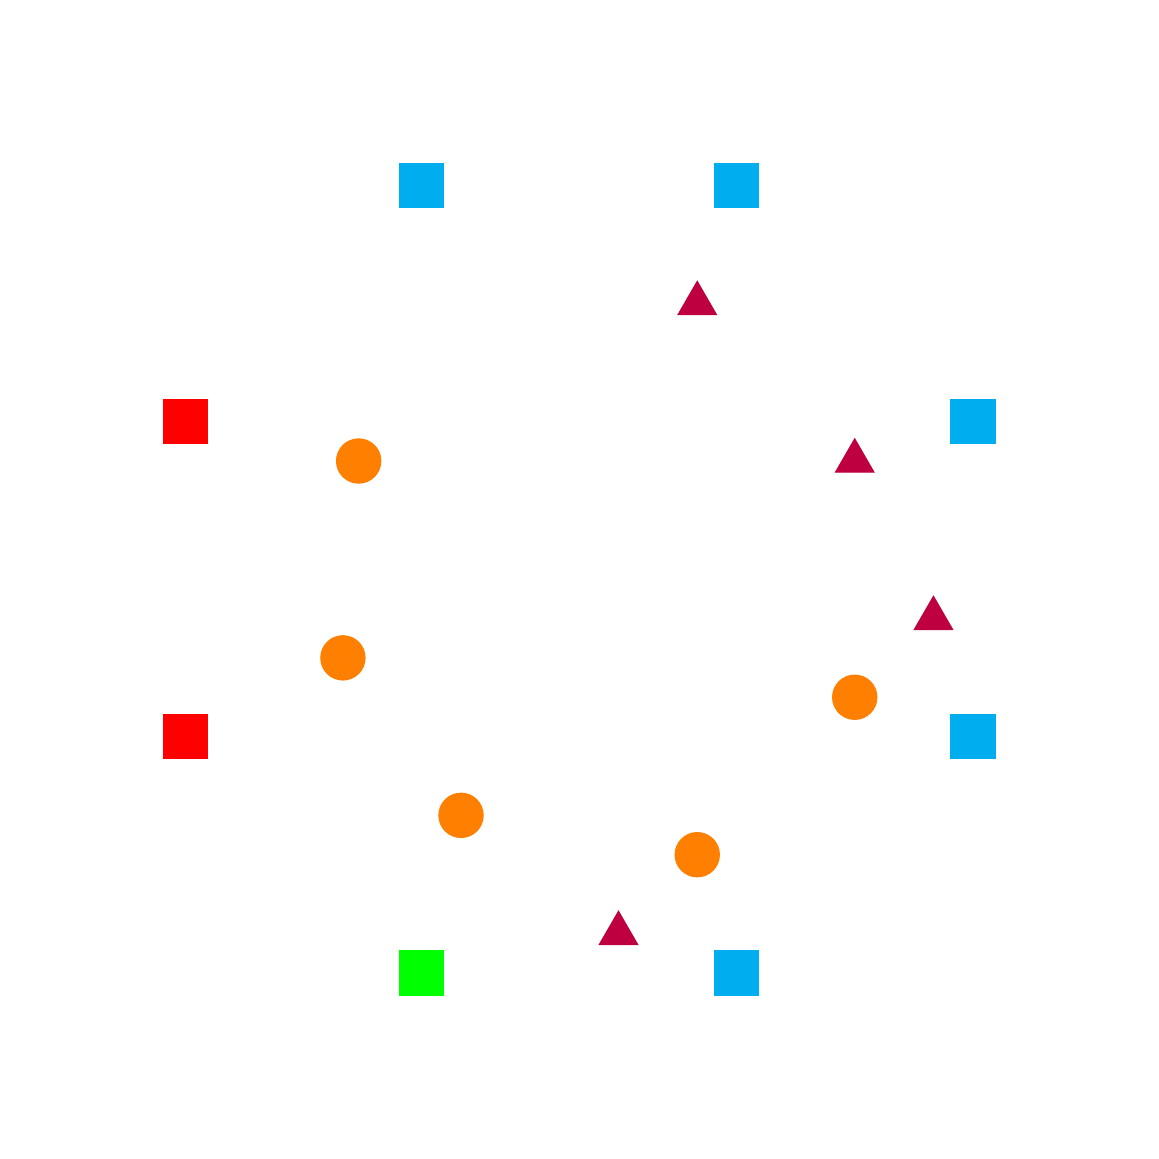
\begin{tikzpicture}
\draw [very thin, white] (0,0) grid (14,14);
\draw [cyan] plot [only marks, mark=square*, mark size=8pt] coordinates {(9,12) (5,12) (12,9) (12,5) (9,2)};
\draw [green] plot [only marks, mark=square*, mark size=8pt] coordinates {(5,2)};
\draw [red] plot [only marks, mark=square*, mark size=8pt] coordinates {(2,5) (2,9)};
\draw [orange] plot [only marks, mark size=8pt, mark=*] coordinates {(4,6) (5.5,4) (4.2,8.5) (8.5,3.5) (10.5,5.5)};
\draw[purple] plot [only marks, mark size=8pt, mark=triangle*] coordinates {(8.5,10.5) (10.5,8.5) (11.5, 6.5) (7.5,2.5)};
\end{tikzpicture}
\end{center}

\newpage

\begin{problem}{1}
What is the probability that the arrow lands on a blue square sector?\\	
\end{problem}

\begin{problem}{2}
What is the probability that the arrow lands on a green square sector?\\	
\end{problem}

\begin{problem}{3}
What is the probability that the arrow lands on a sector without circles and triangles?\\	
\end{problem}

\begin{problem}{4}
What is the probability that the arrow lands on a sector with purple triangles?\\
\end{problem}

\begin{problem}{5}
What is the probability that the arrow lands on a sector with orange circles?\\	
\end{problem}

\begin{problem}{7}
What is the probability that the arrow lands on a sector that contains both orange circles and purple triangles?\\	
\end{problem}

\begin{problem}{8}
What is the probability that the arrow lands on a sector that is either blue or green?	
\end{problem}

\begin{problem}{9}
In problems 1 and 2 you found the separate probabilities for blue and for green sectors. How does your answer from problem 8 compare to these two? Do you think this pattern will always be true when you find the probability of one thing \textbf{OR} another?\\	
\end{problem}

\begin{problem}{10}
Check your intuition from problem 9 and find the probability of landing on a purple triangle or an orange circle. How does this compare to the sum of problems 4 and 5? Did the pattern hold?\\ 	
\end{problem}


\begin{problem}{11}
Why did the addition case work in problem 9 but not in problem 10? What is different about these two problems? Can you think of a rule that would work in both cases?\\	
\end{problem}




\end{document}